\section{User Manual}

We will now see all the possibilities of our web application in details. In order to do that, we will follow the classical path of an ordinary user.

\subsection{The basics: How to create an account and to log in.}

\paragraph{}
When your firstly go on the homepage of the website, you meet a form to log in. As in other applications, you just have to put your credentials to log in. If you want to create a new account, you just have to click on the corresponding button. On the new page, you juste choose your credentials and send them.

\begin{figure}[H]
    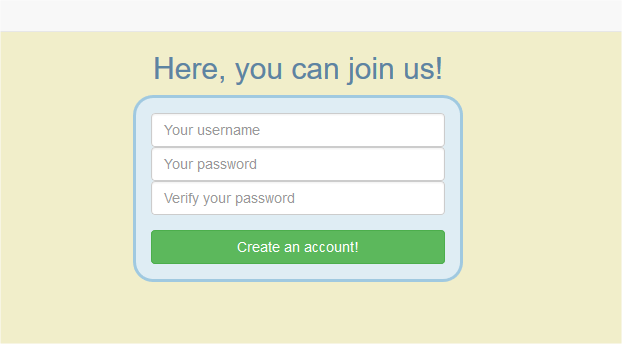
\includegraphics[width=0.5\textwidth]{./images/signin.png}
    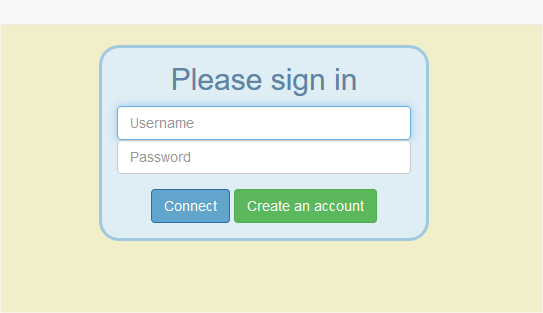
\includegraphics[width=0.5\textwidth]{./images/login.png}
    \caption{Login and signin}
\end{figure}

\paragraph{}
Now that we passed through all the formalities, we can go on the real features of our application!

\subsection{The front page for connected users: The Ali Baba's cave of lessons.}

\paragraph{}
Now that you are connected to your session, the front page is not the same anymore. All the lessons posted by other users that you haven't done are listed here! You can browse to find what you want. The lessons are ordered by creation date, from newer to older. 

\paragraph{}
For each lesson of the list, you can see its title, its difficulty, its theme, the name of the user who posted it and the creation date. The theme of the lesson is the dominant theme according to prevalence of questions. There are three kind of themes : Vocabulary, Grammar and Comprehension. Balanced lessons don't have any dominant theme, there are the same amount of each type of questions.

\paragraph{}
You want something specific? Search filters are here to help you find what you really want! You can search lessons by name, by difficulty and dominant. Of course, you can user several filters at the same time.

\begin{figure}[H]
    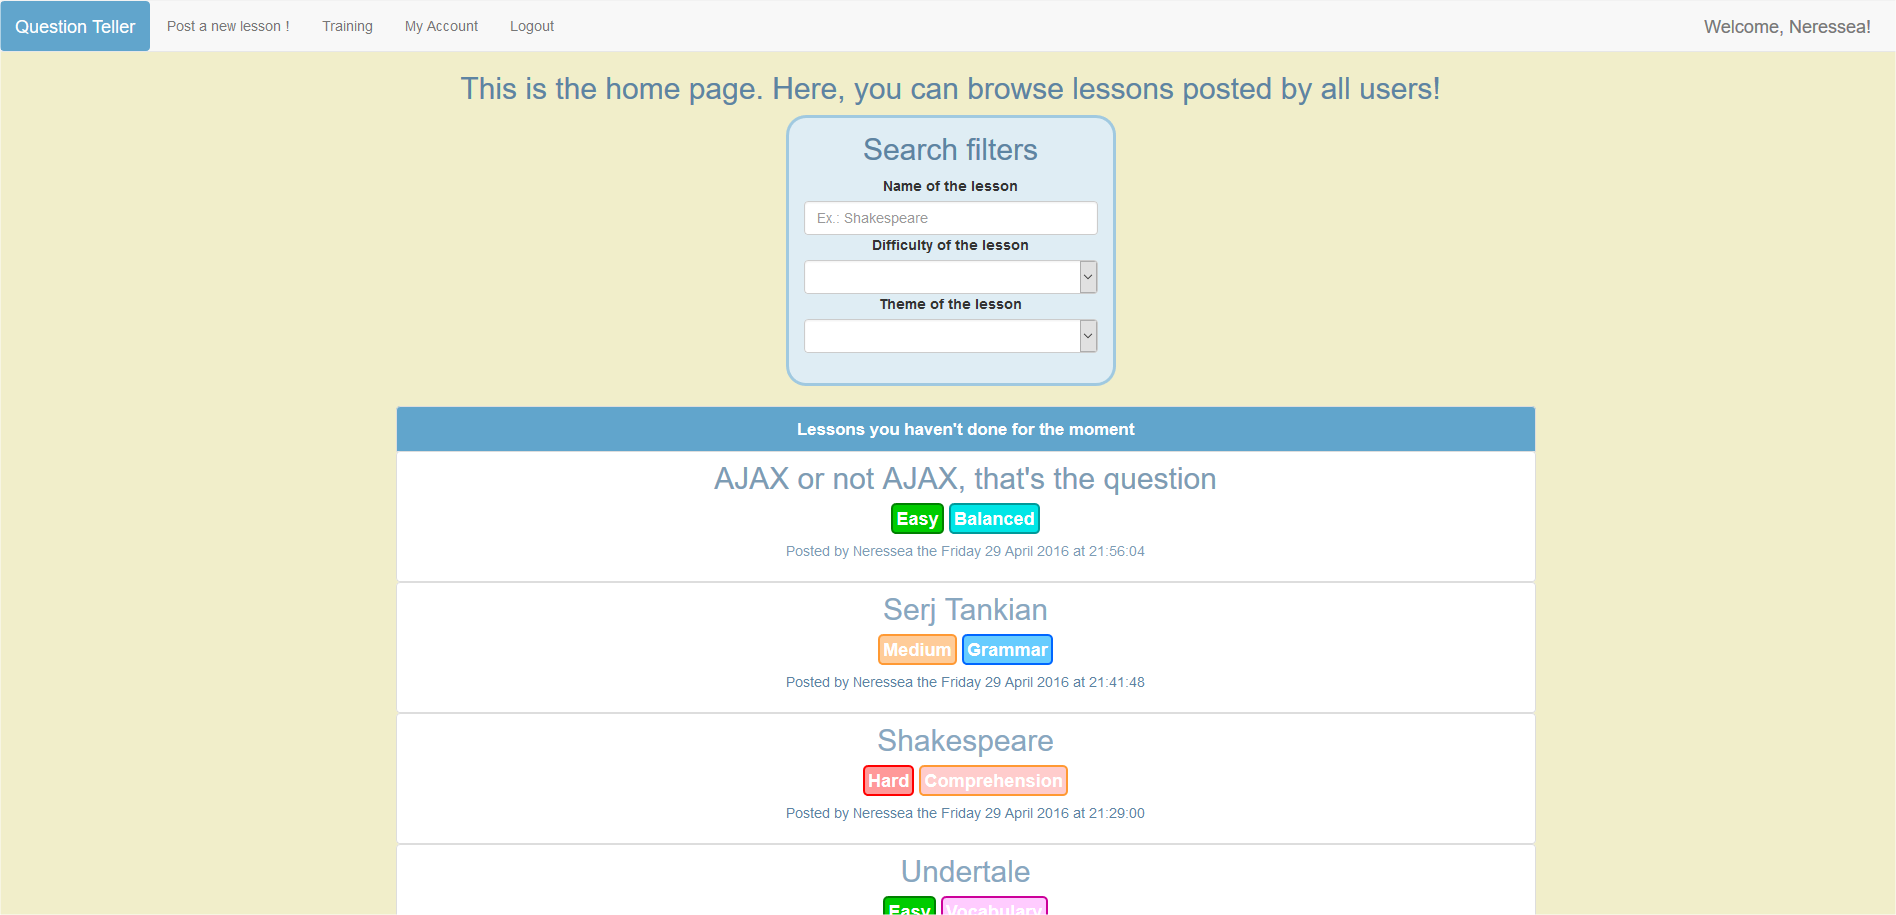
\includegraphics[width=1\textwidth]{./images/snapshot1.png}
    \caption{Front page and search filters}
\end{figure}

\paragraph{}
Now the front page is pretty and all, but we think that you don't want to stay here forever. So you can navigate through sections thanks to the navigation section, or click on a lesson to try it out.

\subsection{Now the real thing: How to try a lesson.}

\paragraph{}
Now that you chose your lesson, the time has come to face it! A lesson can have several stories. A story can be either a text or a youtube video. For each story, the three kind of questions grouped in sections : the first is for vocabulary questions, the second is for grammatical questions and the third is for comprehension questions.

\paragraph{}
In each of these sections, you can have several questions. The vocabulary questions are fill-in-the-blank exercises related to the story, grammatical questions are 4-choices MCQ and finally comprehension questions are direct questions where only one answer is accepted.

\paragraph{}
When you filled all the answers tou know the answer, you can check it. The website will show you the correction of the lesson. If your answer was correct, it is shown in green. If it is wrong, it is shown in red and next to it there is the correct answer in green. \linebreak
At the top of the lesson, you have your statistics for this lesson : the percentage of correct answer for each type of questions. These statistics will be add to your general stats in your account section.

\begin{figure}[H]
    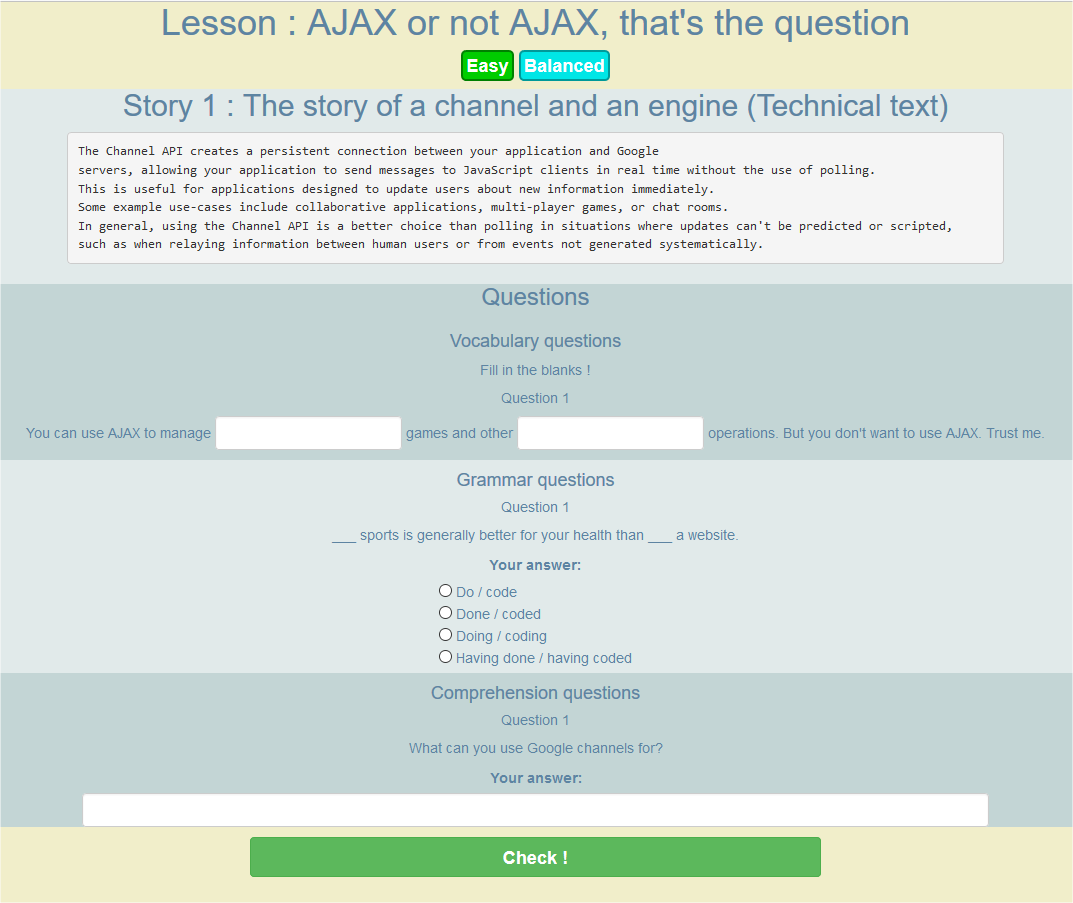
\includegraphics[width=0.5\textwidth]{./images/trylesson.png}
    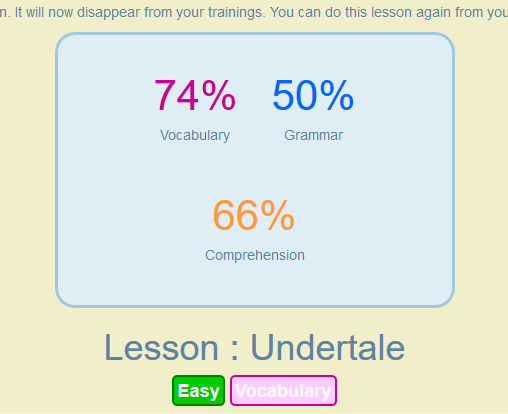
\includegraphics[width=0.5\textwidth]{./images/results.png}
    \caption{When you try out a lesson}
\end{figure}

\subsection{Want to see your progression? You can find everything in your account.}
If you want to track your progress - and if you really want to progress you are likely to do it - you can see it from your account section. \linebreak
Here, you can see at the top of the page your global stats for each type of question. This can help you to know your weaknesses and strengths. Below that, you have the list of all lessons you have already done. These won't show up again in the front page nor in the training program, but you can still access them from here and try them again. \linebreak
But now, what is precisely the training program?

\begin{figure}[H]
    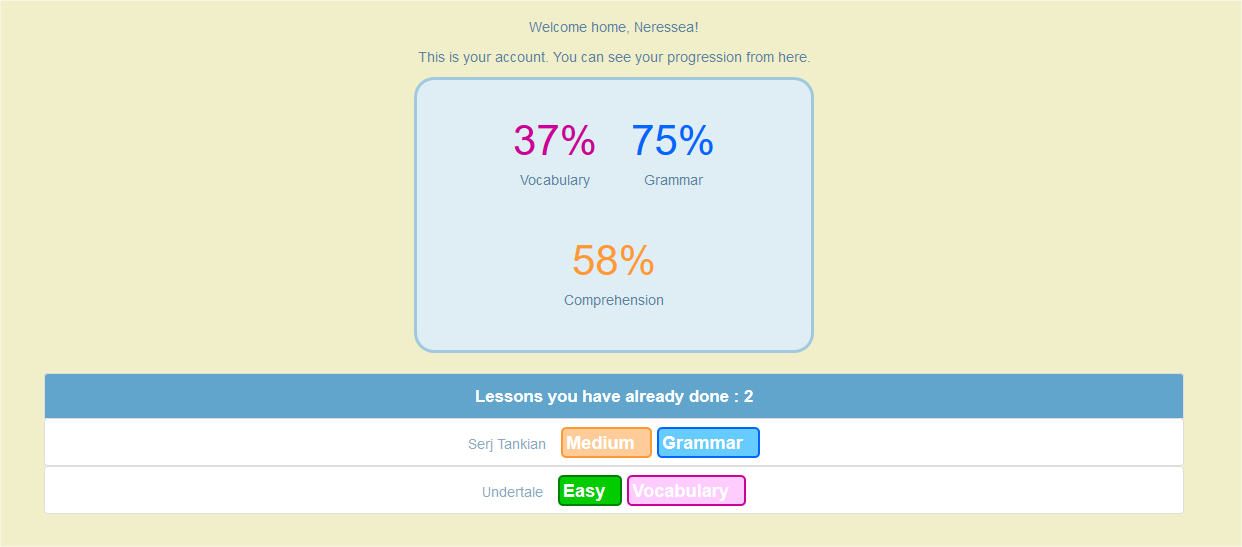
\includegraphics[width=1\textwidth]{./images/account.png}
    \caption{Your account page}
\end{figure}

\subsection{To go further: Let us choose how to train your english!}

\paragraph{}
So, if you go on the "Training" section in the navigation bar, the server will challenge you with a lesson of its own. But it won't choose it from nowhere ; indeed, the server will check what your weaknesses are, and will search for a lesson that can help you to improve your skills in this domain, and that you haven't already done.\linebreak
But if it does not find a lesson that you haven't done, it will at this momentsend you a random lesson. And if you have already done all the lessons of the database, it will just send you an excuse message. However, if you already did everything, I think you already are skilled enough!

\paragraph{}
So now you know about everything as a student user. But what if you want to send your own lesson?

\subsection{Now, you are the teacher: Post a new lesson, and help other students to improve themselves!}

\paragraph{}
If you want to help others, you can also change hats and go to your teacher hat. To do this, you just have to go in the section "Post a new lesson!". Here, you can fill in all the required fields concerning the lesson: its title and the difficulty you think it has. 

\paragraph{}
After that, you can add new stories to the lesson with the related link and fill in them. For each story, you have to choose a title and set the content of the story. Tou can also choose the type of the content (text or youtube video). At the moment you change the content of the story, you have the preview of its display. It is really helpful if you want to listen to the video you want to set while adding questions. You won't have to change of page every time you want to set pause. 

\paragraph{}
After that, you can fill questions. You can add questions to each section (Voca, Grammar, Comprehension) as you wish. Now you just have to fill fields for each question. \linebreak
For vocabulary related questions, you just write the text you want. And to indicate us whiwh words you want to be replaced by a hole, you just surround it with the markers [hole][/hole]. For instance : "Yesterday, I bought [hole]bread[/hole].". In this example, the word "bread" will be replaced by a blank for the user. \linebreak
Regarding the grammar questions, they are all MCQ where you fill in the question and the 4 different answers. The first answer will be the correct one. When it is displayed to the user trying it, the answers are shuffled, of course. \linebreak
And finally, the last kind of question : the comprehension ones. Here, you just have to give us the question and the answer. \linebreak
You can note that the answers of the user must exactly the same for fill-in-the-blank and direct questions. For instance, if the answer you gave is "The answer" when creating the question, "answer" won't be considered as a correct answer. However, it doesn't matter if the answer is uppercased or lowercased. In our example, the answer "THE ANswER" will be considered as correct.

\paragraph{}
Now that you filled in all the fields, you can send us your lesson! And don't worry: the website is kind enough to tell you if you forgot fields. \linebreak
\emph{Now that we saw everything that is possible with our application, we will see how it is done in the code!}

